\documentclass{beamer}
\usetheme{CambridgeUS}
\usepackage{graphicx}

\title{CS6360: Advanced Topics in Machine Learning}
\subtitle{Group Theory $\cap$ Machine Learning}

\author{Pranav K Nayak}
\institute{IIT Hyderabad}
\date{}
\begin{document}
\begin{frame}
  \titlepage
\end{frame}
% \begin{frame}
%   \tableofcontents
% \end{frame}
\section{Assignment 1}
\subsection{HAE Intro}
\begin{frame}{Paper Presentation 1}
  \textbf{Homomorphism Autoencoder: Learning Group Structured Representations from Observed Transitions:}  Hamza Keurti, Hsiao-Ru Pan, Michael Besserve, Benjamin Grewe, Bernhard Sch\"alkopf, \textit{ICML 2023}
  \vspace{5pt}


  The paper attempts to model the effect of interventions as transformations in representation space.

  They assert that this problem can be formulated as a problem of learning a homomorphism between the interventional structure of the world and the model's representations of it. This should allow it to be able to reverse-engineer the effects of potential interventions (transformations) through the knowledge of how its representations change.

\end{frame}
\subsection{Objective}
\begin{frame}{The Learning Problem}
  \begin{columns}
    \begin{column}{.5\textwidth}
        
      \begin{itemize}
        \item $W$ is the latent space from which observations are generated, through the process $g$.
        \item $O$ is the space of observations.
        \item $Z$ is the space of representations, mapped to from $O$ through the \textit{inference process} $h$.
      \end{itemize}
   \end{column} 
    \begin{column}{.5\textwidth}
   \begin{figure}
    \centering
    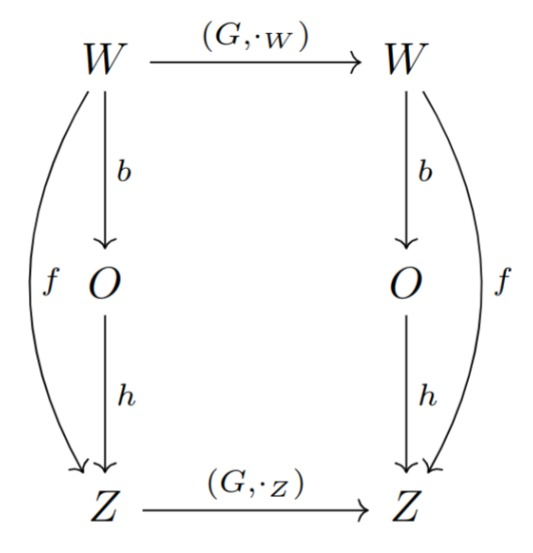
\includegraphics[scale=.3]{group_structure.jpeg}
    \caption{The proposed group structure of the learning problem}
   \end{figure} 
   \end{column} 
  \end{columns}
\end{frame}
\section{Architecture and Loss Propositions}
\begin{frame}{HAE and Two Losses}
  \begin{columns}
    \begin{column}{.6\textwidth}
      \begin{definition}[$N-$step Prediction Loss]
        $\mathcal{L}_{\text{pred}}^N(\rho, h) = \sum_{t}\sum_{j = 1}^{N} || h(o_{t+j}) -  (\prod_{i = 0}^{j-1} \rho(g_{t+i}))h(o_t)||  $
      \end{definition}
      \begin{definition}[$N-$step Reconstruction Loss]
        $\mathcal{L}_{\text{rec}}^N(\rho, h, d) = \sum_{t}\sum_{j = 1}^{N} || o_{t+j} -  d(\prod_{i = 0}^{j-1} \rho(g_{t+i}))h(o_t)||  $
      \end{definition}
   \end{column} 
    \begin{column}{.4\textwidth}
   \begin{figure}
    \centering
    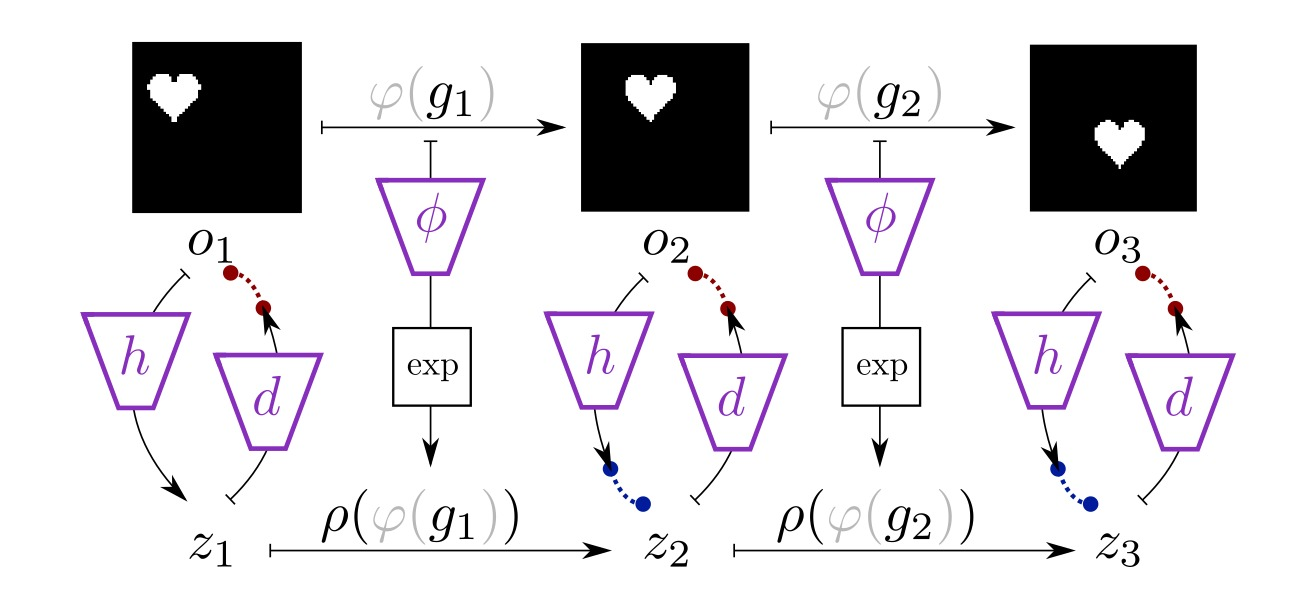
\includegraphics[scale=.1]{hae.jpeg}
    \caption{HAE's Architecture}
   \end{figure} 
   \end{column} 
  \end{columns}
\vspace{10pt}
  A weighted sum of both losses, $\mathcal{L}(\rho, h, d) = \mathcal{L}_{\text{rec}^N}(\rho, h, d) + \gamma \mathcal{L}_{\text{pred}}^N(\rho, h)$, is optimized for.

\end{frame}
\section{Theorem}
\begin{frame}{Restrictions on the Representation Class}
 \begin{theorem}
  If $(\rho, h, d)$ are continuous and minimize the expectation of $\mathcal{L}_{\text{pred}}^2(\rho, h) + \gamma \mathcal{L}_{\text{rec}}^k(\rho, h, d)$, for $k \geq 0$, then $\rho$ is a non-trivial group representation and $(\rho, h)$ is a symmetry-based representation.
 \end{theorem} 
 Informally, a symmetry-based representation is one that satisfies the following: 
 \[ 
 \rho(g_1, g_2, ..., g_n)(z_1 \oplus ... \oplus z_n) = \rho_1(g_1)(z_1)  \oplus ... \oplus \rho_n(g_n)(z_n) \text{~where~} z_i = h(o_i)
 .\]
\end{frame}
\end{document}
